\documentclass[a4paper]{article}
\ifdefined\HCode
\def\pgfsysdriver{pgfsys-tex4ht.def}
\fi
\usepackage{fullpage}
\title{Offsetting parameterised Bezier curves}
\author{Simon Cozens}
\usepackage{amsmath}
\usepackage{mathtools}

\newtagform{brackets}{[}{]}
\usetagform{brackets}
\usepackage{breqn}
\newcommand{\icol}[1]{% inline column vector
  \left(\begin{smallmatrix}#1\end{smallmatrix}\right)%
}
\newcommand{\Norm}[1]{\lVert #1 \rVert}
\newcommand{\norm}[1]{\lvert #1 \rvert}

\usepackage{tikz}
\newcommand\DrawControl[3]{
  node[#2,circle,fill=#2,inner sep=1pt,label=#3] at #1 {}
}
\begin{document}
\maketitle

A common problem in type design is the creation of pairs of curves representing the stroke of a pen: an inner curve and an outer curve delimit the contours of a writing implement of fixed or flexible thickness. While it is impossible to precisely offset a Bezier curve at a given width, this paper presents a simple approximation by minimizing the error between desired distance and actual distance. This can also be applied to situations where the thickness varies linearly across the width of the curve.

We use a simplification due to Tunni, who postulates that any curve $\mathbf{a,b,c,d}$ with straight handles (i.e. where the control points $\mathbf{b}$ and $\mathbf{c}$ are positioned orthogonally to $\mathbf{a}$ and $\mathbf{d}$respectively) can be represented in terms of start and end points $\mathbf{a}$ and $\mathbf{d}$ and a curve tension $\tau$. To determine curve tension, compute the point $\mathbf{T}$ where $\vec{\mathbf{ab}}$ intersects $\vec{\mathbf{cd}}$:

\bigskip
\resizebox{100pt}{!}{
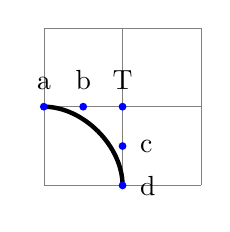
\begin{tikzpicture}[baseline]
\draw[help lines] (0,0) grid (2,2);
\draw[ultra thick] 
  (1,0) 
    .. controls (1,0.5) and (0.5,1) .. 
  (0,1) \DrawControl{(1,0.5)}{blue}{right:c}\DrawControl{(0.5,1)}{blue}{b} \DrawControl{(1,1)}{blue}{T}\DrawControl{(1,0)}{blue}{right:d}\DrawControl{(0,1)}{blue}{a};
\end{tikzpicture}
}
\bigskip

The curve tension is given by the mean of the ratios $\frac{\Norm{\mathbf{ab}}}{\Norm{\mathbf{aT}}}$ and $\frac{\Norm{\mathbf{dc}}}{\Norm{\mathbf{dT}}}$. Given the points $\mathbf{a,d}$ and a tension $\tau$ we can compute the Bezier control points $\mathbf{b,c}$ by setting them at the appropriate ratios.

This conceptualization enables us to find similar parameters for an offset Bezier curve. We will approach the problem in small pieces, demonstrating the technique first before solving the general case.

\section{Outer offset of a unit Bezier curve}

Consider first the unit Bezier curve $\mathbf{B_A}$ with $\mathbf{a} = (0, 1), \mathbf{d} = (1, 0)$ and $\mathbf{c}$ and $\mathbf{d}$ chosen as orthogonal control points with a curve tension $\alpha$. What are the parameters for a Bezier curve $\mathbf{B_B}$ offsetting this curve on the outside at a fixed distance $\delta$?

\bigskip
\resizebox{100pt}{!}{
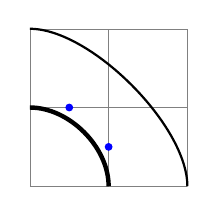
\begin{tikzpicture}[baseline]
\draw[help lines] (0,0) grid (2,2);
\draw[ultra thick] 
  (1,0) 
    .. controls (1,0.5) and (0.5,1) .. 
  (0,1) \DrawControl{(1,0.5)}{blue}{}\DrawControl{(0.5,1)}{blue}{} ;  
\draw[thick](2,0) .. controls (2,0.77) and (0.77,2) .. (0,2);
\end{tikzpicture}
}
\bigskip

Clearly we have $\mathbf{a} = (0, 1+\delta), \mathbf{d} = (1+\delta, 0)$, so it remains to find the curve tension $\beta$.

As a function of time, the distance between the two curves is:

\begin{equation}\Norm{\mathbf{B_A}(t)\cdot\mathbf{B_B}(t)}\end{equation}

and at any point on the curve, the expected distance is $\delta$. Knowing
it is impossible to achieve a perfect offset, we can treat this as an optimization problem: find the value of $\beta$ which minimizes the total error function

\begin{equation}\int_{0}^{1} (\Norm{\mathbf{B_A}(t)\cdot\mathbf{B_B}(t)} - \delta)^2 dt\end{equation}

This integral turns out to be tricky to compute due to the presence of the square root, so instead we create an equivalent error function using the square of the distance. We expect the square of the distance to be $\delta^2$, and we square the difference of these two values to perform a least squares optimization. This leads to an error function of

\begin{equation}(\norm{\mathbf{B_A}(t)\cdot\mathbf{B_B}(t)} - \delta^2)^2\end{equation}

For a unit Bezier, we have:

\begin{multline}
\mathbf{B_A}(t) = \left(\begin{matrix}
t^3+3 (1-t) t^2+3 \alpha  (1-t)^2 t \\
3 \alpha  t^2 (1-t)+(1-t)^3+3 t (1-t)^2
\end{matrix}\right)\\
\mathbf{B_B}(t) = \left(\begin{matrix}
(\Delta +1) t^3+3 (1-t) t^2 ((1-\beta ) (\Delta +1)+\beta  (\Delta +1))+3 \beta  (\Delta +1) (1-t)^2 t \\
3 \beta  (\Delta +1) t^2 (1-t)+3 t (1-t)^2 ((1-\beta ) (\Delta +1)+\beta  (\Delta +1))+(\Delta +1) (1-t)^3
\end{matrix}\right) \\
= \left(\begin{matrix}
(\Delta +1) t \left(3 \beta  (t-1)^2+t (3-2 t)\right) \\
(\Delta +1) (-(t-1)) \left((3 \beta -2) t^2+t+1\right)
\end{matrix}
\right)
\end{multline}

leading to a square distance

\begin{multline}\norm{\mathbf{B_A}(t)\cdot\mathbf{B_B}(t)} = 
t^2 \left(3 \alpha  (t-1)^2-3 \beta  (\Delta +1) (t-1)^2+\Delta  t (2 t-3)\right)^2+ \\ (t-1)^2 (\Delta +t (\Delta +t (-3 \alpha +3 \beta  (\Delta +1)-2 \Delta )))^2
\end{multline}

and therefore an error function

\begin{dmath}E(\mathbf{B_A},\mathbf{B_B}) = \int_{0}^{1}(\norm{\mathbf{B_A}(t)\cdot\mathbf{B_B}(t)} - \delta^2)^2 dt = \frac{1}{30030}\left(
1161 (\alpha -\beta )^4 - 36 (129 \beta +148) \delta  (\alpha -\beta )^3 + 18 \left(387 \beta ^2+888 \beta +146\right) \delta ^2 (\alpha -\beta )^2 - 4 (9 \beta  (3 \beta  (43 \beta +148)+146)-2138) \delta ^3 (\alpha -\beta ) (\beta  (9 \beta  (\beta  (129 \beta +592)+292)-8552)+2916) \delta ^4\right)
\end{dmath}

This looks horrific, but it's only a quartic, and is easily optimizable. Rather than solving the differential equation for the general case, let's be practical, remember that $\alpha$ and $\delta$ will be given and go for a numerical method to minimize the error function.

Beginning with $\beta_1 = \alpha$ and applying the Newton-Raphson optimization method gives us an iterated function

\begin{multline}
\beta_{n+1} = \beta_n -\frac{E'(\mathbf{B_A},\mathbf{B_B})}{E''(\mathbf{B_A},\mathbf{B_B})} \\
= \beta_n - 
\frac{
\left(\begin{matrix}
-36 \left(387 \beta ^2+888 \beta +146\right) \delta ^2 (\alpha -\beta ) \\
-4 (9 \beta  (129 \beta +3 (43 \beta +148))+9 (3 \beta  (43 \beta +148)+146)) \delta ^3 (\alpha -\beta ) \\
+18 (774 \beta +888) \delta ^2 (\alpha -\beta )^2-4644 \delta  (\alpha -\beta )^3+108 (129 \beta +148) \delta  (\alpha -\beta )^2 \\
-4644 (\alpha -\beta )^3+(9 \beta  (\beta  (129 \beta +592)+292)+ \\
\beta  (9 \beta  (258 \beta +592)+9 (\beta  (129 \beta +592)+292))-8552) \delta ^4+4 (9 \beta  (3 \beta  (43 \beta +148)+146)-2138) \delta ^3
\end{matrix}\right)
}{\left(\begin{matrix}
-4 (2322 \beta +18 (129 \beta +3 (43 \beta +148))) \delta ^3 (\alpha -\beta )+ \\
13932 \delta ^2 (\alpha -\beta )^2-72 (774 \beta +888) \delta ^2 (\alpha -\beta )+27864 \delta  (\alpha -\beta )^2\\
-216 (129 \beta +148) \delta  (\alpha -\beta )+\\
13932 (\alpha -\beta )^2+36 \left(387 \beta ^2+888 \beta +146\right) \delta ^2+\\
(\beta  (2322 \beta +18 (258 \beta +592))+2 (9 \beta  (258 \beta +592)+9 (\beta  (129 \beta +592)+292))) \delta ^4 + \\
8 (9 \beta  (129 \beta +3 (43 \beta +148))+9 (3 \beta  (43 \beta +148)+146)) \delta ^3
\end{matrix}\right)}
\end{multline}

quickly converges to the minimum error, giving us the optimal curve tension.

As an example, plugging in $\alpha = 0.55, \Delta = 1$:

\begin{align*}
\beta_1 = 0.55 \\
\beta_2 = 0.550987 \\
\beta_3 = 0.550985 \\
\beta_4 = 0.550985
\end{align*}

\subsection{We can cheat}

Thankfully, we find by inspection that the optimal value of $\beta$ given $\alpha$ and $\Delta$, $\beta(\alpha, \Delta)$ turns out to be pretty much linear in both $\alpha$ and $\Delta$ when $\alpha \ge 0.3$. A very pleasing result is:

\begin{dmath}
\beta(\alpha,1) = 0.275985 + \frac{\alpha}{2}
\end{dmath}

Note that this gives exactly the answer given by our Newton-Raphson method above. A more general, but less accurate, approximation is:

\begin{dmath}\label{approx}
\beta(\alpha, \delta) = 0.513216 \alpha -0.025407 \delta+0.296638
\end{dmath}

\section{Inner offsetting of a unit Bezier}

What if we want to go the other way, and find the inner curve at a fixed distance?

\bigskip
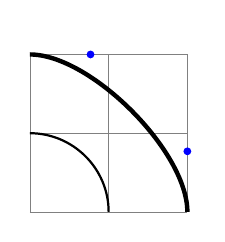
\begin{tikzpicture}[baseline]
\draw[help lines] (0,0) grid (2,2);
\draw[ultra thick] 
  (2,0) 
    .. controls (2,0.77) and (0.77,2) .. 
  (0,2) \DrawControl{(2,0.77)}{blue}{}\DrawControl{(0.77,2)}{blue}{} ;  
\draw[thick](1,0) .. controls (1,0.55) and (0.55,1) .. (0,1);
\end{tikzpicture}
\bigskip

A very similar pattern applies, but this time we construct $\mathbf{B_B}$ as
$\mathbf{a} = (0, 1-\delta, \mathbf{d} = (1-\delta, 0)$
and the Newton step $\frac{E'(\mathbf{B_A},\mathbf{B_B})}{E''(\mathbf{B_A},\mathbf{B_B})}$ is

\begin{dmath}
\frac{\left(
\begin{matrix}
18 \alpha ^2 \left(414 \beta  (\delta -1)^2+244 (\delta -1)^2\right)+8 \alpha  \left(1098 \beta  (\delta -1)^2-108 (\delta -1)^2\right)+ \\
4644 \beta ^3 (\delta -1)^4+15984 \beta ^2 (\delta -1)^4+72 \beta  \left(73 \delta ^2-718 \delta +548\right) (\delta -1)^2 \\
-8 \left(1069 \delta ^2+3439 \delta -4011\right) (\delta -1)^2
\end{matrix}\right)
}{\left(
  \begin{matrix}7452 \alpha ^2 (\delta -1)^2+8784 \alpha  (\delta -1)^2+13932 \beta ^2 (\delta -1)^4+31968 \beta  (\delta -1)^4+ \\
  72 \left(73 \delta ^2-718 \delta +548\right) (\delta -1)^2
  \end{matrix}\right)
}
\end{dmath}

Equally, we can invert our approximation \ref{approx} above, giving:

\begin{equation}
\alpha = 1.9485 \beta + 0.0495055 \delta -0.577999
\end{equation}

\section{Outer offsetting of an arbitrary normalized curve}

Real-world curves are not unit curves $(0, 1)\cdots(1, 0)$. However, we can always use affine transformation to locate the start at $\mathbf{a} = (1, 0)$, leaving the end at $\mathbf{d} = (0, x)$. The control points for a Bezier curve with tension $\tau$ $\mathbf{B_A}$ would then be set at $\mathbf{b} = (1-\tau, 0), \mathbf{c} = (0, x(1-\tau))$. The problem, again, is to find the offset curve $\mathbf{B_B}$ which best approximates a fixed distance $\delta$ from $\mathbf{B_A}$.

Now we have $\mathbf{a} = (0, 1+\delta), \mathbf{d} = (x+\delta, 0)$. Following exactly the procedure above, $\norm{\mathbf{B_A}(t)\cdot\mathbf{B_B}(t)}$, the square of the distance between the two curves at point $t$, is

\begin{dmath}
t^2 \left(\delta  \left(t (2 t-3)-3 \beta  (t-1)^2\right)+3 (t-1)^2 x (\alpha -\beta )\right)^2+(t-1)^2 (\delta +t (\delta +t (-3 \alpha +3 \beta  (\delta +1)-2 \delta )))^2
\end{dmath}

and the total error across the curve is

\begin{dmath}E(\mathbf{B_A},\mathbf{B_B}) = \int_{0}^{1}(\norm{\mathbf{B_A}(t)\cdot\mathbf{B_B}(t)} - \delta^2)^2 dt =
\frac{
\begin{matrix}27 \left(14 x^4+15 x^2+14\right) (\alpha -\beta )^4-9 \delta  (x+1) (\alpha -\beta )^3 (3 (56 \beta +45)+x (-78 \beta +3 (56 \beta +45) x+26)) \\
+ 9 \delta ^2 (\alpha -\beta )^2 \left(566 \beta +9 \beta ^2 (x (33 x+20)+33)+2 \beta  x (283 x+322)+4 x (85-6 x)-24\right) \\
+ 2 (9 \beta  (3 \beta  (43 \beta +148)+146)-2138) \delta ^3 (x+1) (\alpha -\beta ) \\
+ (\beta  (9 \beta  (\beta  (129 \beta +592)+292)-8552)+2916) \delta ^4
\end{matrix}
}{30030}
\end{dmath}

Once again, it's only a quartic and three of the variables are given. We can apply the Newton-Raphson method again, giving:

\begin{multline}
\beta_{n+1} = \beta_n -\frac{E'(\mathbf{B_A},\mathbf{B_B})}{E''(\mathbf{B_A},\mathbf{B_B})} = \beta_n - \\
\frac{\begin{matrix}4 \left(1161 \beta ^3+3996 \beta ^2+1314 \beta -2138\right) \delta ^4\\
-54 \delta  (x+1) \left(28 x^2-13 x+28\right) (\alpha -\beta )^3-108 \left(14 x^4+15 x^2+14\right) (\alpha -\beta )^3 \\
-18 \left(387 \beta ^2+888 \beta +146\right) \delta ^3 (x+1) (\alpha -\beta ) \\
-18 \delta ^2 (\alpha -\beta ) \left(566 \beta +9 \beta ^2 (x (33 x+20)+33)+2 \beta  x (283 x+322)+4 x (85-6 x)-24\right)+ \\
9 \delta ^2 (\alpha -\beta )^2 (18 \beta  (x (33 x+20)+33)+2 x (283 x+322)+566) \\
+27 \delta  (x+1) (\alpha -\beta )^2 (3 (56 \beta +45)+x (-78 \beta +3 (56 \beta +45) x+26))+ \\
2 (9 \beta  (3 \beta  (43 \beta +148)+146)-2138) \delta ^3 (x+1)\end{matrix}}{\begin{matrix}
18 \left(2 \left(387 \beta ^2+888 \beta +146\right) \delta ^4+18 \delta  (x+1) \left(28 x^2-13 x+28\right) (\alpha -\beta )^2+18 \left(14 x^4+15 x^2+14\right) \right. \\
\left. (\alpha -\beta )^2 -6 (129 \beta +148) \delta ^3 (x+1) (\alpha -\beta )+9 \delta ^2 (x (33 x+20)+33) (\alpha -\beta )^2-2 \delta ^2 (\alpha -\beta ) \right. \\
\left. (18 \beta  (x (33 x+20)+33)+2 x (283 x+322)+566)-3 \delta  (x+1) (\alpha -\beta ) (3 (56 \beta +45)+ \right.\\
\left.x (-78 \beta +3 (56 \beta +45) x+26))+ 2 \left(387 \beta ^2+888 \beta +146\right) \delta ^3 (x+1)+\delta ^2 \left(566 \beta +9 \beta ^2 (x (33 x+20)+33)+ \right. \right. \\
\left. \left. 2 \beta  x (283 x+322)+4 x (85-6 x)-24\right)\right)\end{matrix}}
\end{multline}

By iterating this approximation, we can derive the tension for a curve at an offset of a given distance $\delta$ from an arbitrary Bezier curve specified by two points and a curve tension parameter.

But wait, it gets more complicated.

\section{Offsetting at a linear-gradiated distance}

Strokes in fonts often have a feature called \textit{contrast}, meaning that the horizontal offset is not the same as the vertical offset:

\bigskip
\resizebox{150pt}{!}{
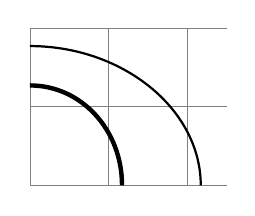
\begin{tikzpicture}
\draw[help lines] (0,0) grid (2.5,2);
\draw[ultra thick] 
  (0,1.27) .. controls (0.65,1.27) and (1.17, 0.71) .. (1.17,0);
\draw[thick](0,1.77) .. controls (1.18,1.77) and (2.17,0.97) .. (2.17,0);
\end{tikzpicture}
}
\bigskip

To model this we will assume that the desired distance between curves is a linear function of curve time $t$:

\begin{equation}
\delta(t) = \delta_s(1-t) + \delta_e t
\end{equation}

And now our error function is 
\begin{dmath}
(\norm{\mathbf{B_A}(t)\cdot\mathbf{B_B}(t)} - \delta(t)^2)^2 = x
\end{dmath}

The total integrated error across the curve becomes\dots\ very complicated, but computable. We can apply a similar Newton-Raphson method as above, leading to the functions given in the associated Python script.

\end{document}
